% 第 1 章 Getting Started With the GUI
\bichapter{使用 GUI 入门}{Getting Started With the GUI}
\label{chap:gui-start}

IC Compiler II 图形用户界面（GUI）提供灵活的工作环境，可用多个窗口执行不同任务。这些 GUI 窗口在 X Window 环境中彼此独立运行，但共享工具中的块（block）数据与全局选择数据。

下列主题说明如何使用 GUI：
\begin{itemize}
  \item 启动 GUI
  \item 关闭 GUI
  \item 从 GUI 退出工具
  \item 在无 X 服务器时以批处理模式运行 GUI
  \item 在脚本中判断 GUI 是否正在运行
  \item 使用 GUI 窗口
  \item 截取工具窗口的屏幕截图
  \item 使用控制台
  \item 设置应用程序首选项
  \item 使用命令搜索
  \item 使用主题搜索
  \item 查看每日提示
  \item 创建参考方法学脚本
  \item 查看与编辑应用选项
  \item 在块窗口中工作
  \item 更改物理设计的视图
  \item 编辑物理版图
  \item 查看金属填充数据
\end{itemize}

% ============================================================
\section{启动 GUI}
\subsection*{Starting the GUI}

IC Compiler II GUI 同时提供菜单命令与命令行界面（CLI）。它是高级分析与物理编辑工具。某些任务只能从 GUI 完成，例如准确显示块，以及提供可视化分析工具。IC Compiler II GUI 的外观与操作方式和其他 Synopsys GUI 一致。

IC Compiler II GUI 使用 \cmd{DISPLAY} 环境变量确定显示位置。使用 GUI 之前，请确认该变量已设为你的 UNIX 或 Linux 系统显示器名称，并确认 \cmd{bin} 目录的路径已包含在 \cmd{PATH} 变量中。

要在 GUI 模式下启动 IC Compiler II 工具，请在 UNIX 或 Linux shell 中输入带 \opt{-gui} 选项的 \cmd{icc2\_shell} 命令：
\begin{lstlisting}
% icc2_shell -gui
\end{lstlisting}

要启动 Library Manager 工具的 GUI，请按如下方式使用带 \opt{-gui} 选项的 \cmd{icc2\_lm\_shell} 命令：
\begin{lstlisting}
% icc2_lm_shell -gui
\end{lstlisting}

启动 IC Compiler II GUI 时，还可以在命令行上加入其他选项。例如可以使用：
\begin{itemize}
  \item \opt{-help}：显示全部可用选项的列表
  \item \opt{-f} \cmd{script\_file\_name}：执行脚本
  \item \opt{-x} \cmd{command}：执行一条 \cmd{icc2\_shell} 命令
\end{itemize}

启动 GUI 时，工具依次执行下列操作：
\begin{enumerate}
  \item \textbf{运行 setup 文件中的命令。}\\
        IC Compiler II 工具加载 \cmd{.synopsys\_icc2.setup} 与 \cmd{.synopsys\_icc2\_gui/setup.tcl}；Library Manager 工具加载 \cmd{.synopsys\_icc2\_lm.setup} 与 \cmd{.synopsys\_icc2\_lm\_gui/setup.tcl}。工具先运行主目录中的 setup 文件，再运行你执行 \cmd{icc2\_shell} 或 \cmd{icc2\_lm\_shell} 命令时所在本地目录中的文件。
  \item \textbf{运行 \opt{-x} 选项指定的命令，或 \opt{-f} 选项指定的脚本。}
  \item \textbf{打开显示启动画面（splash screen）的主窗口。}\\
        默认情况下，控制台（console）停靠（dock）在主窗口中、状态栏（status bar）上方。
\end{enumerate}

在 CLI 中启动工具并打开块时，IC Compiler II 工具执行相同的启动任务。

若启动任一工具时未打开 GUI，可在命令提示符下输入 \cmd{gui\_start} 命令来打开 GUI：
\begin{lstlisting}
gui_start
\end{lstlisting}

若要在打开 GUI 之前执行脚本，使用 \opt{-file} 选项。例如：
\begin{lstlisting}
gui_start -file my_gui_setup.tcl
\end{lstlisting}

若在 \cmd{icc2\_shell} 提示符下打开块后再打开 GUI，IC Compiler II 工具会自动打开一个块窗口（Block window），并在版图视图（layout view）中显示该块。若打开 GUI 时已有多个块处于打开状态，工具会为每个块分别打开一个 Block window。活动窗口（拥有鼠标焦点的窗口）是当前块所在的窗口。

IC Compiler II GUI 为多数图形功能提供菜单命令与对话框，例如在版图视图中查看、选择和高亮对象。菜单命令按功能分组，位于每个 GUI 窗口的菜单中。

% ============================================================
\section{关闭 GUI}
\subsection*{Closing the GUI}

会话期间可以随时打开或关闭 GUI。例如，若需要节省系统资源，可以关闭 GUI，并在 \cmd{icc2\_shell} 或 \cmd{icc2\_lm\_shell} 中继续会话。

要关闭 GUI，执行下列操作之一：
\begin{itemize}
  \item 在 Block window 中选择 \textbf{File > Close GUI}。
  \item 输入 \cmd{gui\_stop} 命令。
\end{itemize}
\begin{lstlisting}
gui_stop
\end{lstlisting}

准备再次使用 GUI 时，在命令行上输入 \cmd{gui\_start} 命令。

% ============================================================
\section{从 GUI 退出工具}
\subsection*{Exiting the Tool From the GUI}

可以随时结束会话并退出 IC Compiler II 或 Library Manager 工具。要退出工具，输入 \cmd{exit} 或 \cmd{quit} 命令，或选择 \textbf{File > Exit}。输入 \cmd{quit!} 命令可退出并忽略工具发出的任何提示。

GUI 处于打开状态时，工具行为取决于是否存在任何已打开块的未保存更改。
\begin{itemize}
  \item 若任何已打开的块中有未保存的更改，将出现 \textbf{Exit IC Compiler II} 对话框或 \textbf{Exit Library Manager} 对话框，供你把更改保存到已修改的块。
  \item 若没有未保存的块更改，则出现消息框，而不是 \textbf{Exit IC Compiler II} 对话框或 \textbf{Exit Library Manager} 对话框。若看到该消息框，单击 OK 即可退出。
\end{itemize}

\begin{noteBox}
退出时工具不保存视图设置。若已更改版图视图或原理图视图（schematic view）的视图设置并希望保存，请在退出工具之前保存，如后文「设置并保存视图属性（Setting and Saving View Properties）」所述。
\end{noteBox}

% ============================================================
\section{在无 X 服务器时以批处理模式运行 GUI}
\subsection*{Running the GUI in Batch Mode Without an X Server}

工具支持一种模式，使你无需运行 X 服务器即可执行与 GUI 相关的命令。使用 \opt{-batch} 选项运行 \cmd{icc2\_shell} 时，若同时指定 \opt{-gui} 选项或 \cmd{start\_gui} 命令，GUI 可以以无界面（headless）模式运行，该模式不需要 X 服务器或显示窗口。在此模式下，通过 \opt{-file} 选项指定的脚本文件向工具提供 Tcl 命令，或用 \opt{-x} 选项在命令行上指定命令。

例如，下列脚本加载设计、创建版图屏幕截图并退出工具：
\begin{lstlisting}
# capture_layout.tcl
open_block ./orca:orca.design
start_gui
gui_write_window_image -file ./layout.png -size {1000 1000} \
   -window [gui_get_current_window -types Layout -mru] -format png
quit!
\end{lstlisting}

要在 headless 模式下运行该脚本，按下列示例指定 \opt{-batch} 选项，后接 \opt{-f} 或 \opt{-x} 选项：
\begin{lstlisting}
% icc2_shell -batch -f capture_layout.tcl
% icc2_shell -batch -x "source capture_layout.tcl"
% icc2_shell -batch \
   -x 'open_block ./orca:orca.design; start_gui; \
   gui_write_window_image -file ./layout.png -format png; \
   quit!'
\end{lstlisting}

除 \opt{-batch} 选项外，还可以用下列命令与选项在 headless 模式下运行工具：
\begin{itemize}
  \item 对 \cmd{gui\_start} 命令指定 \opt{-offscreen 1} 选项。
\end{itemize}
\begin{lstlisting}
# capture_layout.tcl using gui_start -offscreen 1
open_block ./orca:orca.design
start_gui -offscreen 1
gui_write_window_image -file ./layout.png -size {1000 1000} \
   -window [gui_get_current_window -types Layout -mru] -format png
quit!
\end{lstlisting}
\begin{itemize}
  \item 将应用选项 \appopt{gui.batch\_x\_display} 设为 \cmd{offscreen}。
\end{itemize}
\begin{lstlisting}
# capture_layout.tcl using gui.batch_x_display offscreen
open_block ./orca:orca.design
set_app_options -list {gui.batch_x_display offscreen}
start_gui
gui_write_window_image -file ./layout.png -size {1000 1000} \
   -window [gui_get_current_window -types Layout -mru] -format png
quit!
\end{lstlisting}

在每个示例中，工具执行命令时不显示 GUI 窗口，也不需要正在运行的 X 服务器。

% ============================================================
\section{在脚本中判断 GUI 是否正在运行}
\subsection*{Determining Whether the GUI is Running in a Script}

若计划从脚本中执行 GUI 命令，使用应用变量 \cmd{in\_gui\_session} 判断 GUI 是否处于活动状态。GUI 活动时该变量为 \cmd{true}，不活动时为 \cmd{false}，如下例所示：
\begin{lstlisting}
icc2_shell> gui_start
icc2_shell> get_app_var in_gui_session
true
icc2_shell> gui_stop
To restart the GUI, type 'gui_start'.
icc2_shell> get_app_var in_gui_session
false
\end{lstlisting}

% ============================================================
\section{使用 GUI 窗口}
\subsection*{Using GUI Windows}

每个顶层 GUI 窗口在视图窗口中显示设计信息，并提供菜单与对话框（含键盘快捷键）、工具栏与面板、交互式鼠标按钮工具、命令控制台（带命令行界面）以及状态栏。

IC Compiler II GUI 提供下列类型的窗口：
\begin{itemize}
  \item 块窗口（Block window）
  \item 时钟树分析窗口（Clock tree analysis window）
  \item 消息浏览器窗口（Message browser window）
  \item 相对布局窗口（Relative placement (RP) window）
  \item 时序分析窗口（Timing analysis window）
\end{itemize}

每个顶层 GUI 窗口独立于其他 GUI 窗口。标题栏显示产品名称（IC Compiler II）、窗口名称（启动 GUI 时出现的窗口为 \cmd{BlockWindow.1}）、当前任务，以及当前库与块的名称。在一个窗口中选择的设计对象会自动在其他窗口中被选中。

可以打开和关闭 GUI 窗口，也可以打开每种窗口的多个实例，以便使用不同的块设置。每个窗口实例都有唯一名称，其中包含递增的编号。

要打开 GUI 窗口的新实例，选择 \textbf{Window >} \textit{window-type}。

要关闭 GUI 窗口，在要关闭的窗口中选择 \textbf{Window > Close Window}。

\begin{noteBox}
若关闭全部已打开的 GUI 窗口，GUI 会话结束，但你仍留在 \cmd{icc2\_shell} 中，块仍保持打开。可以使用 \cmd{gui\_start} 命令重新打开 GUI。
\end{noteBox}

可以使用 UNIX 或 Linux 桌面上的窗口管理工具移动、调整大小、最小化或最大化 GUI 窗口。

下列主题说明 GUI 窗口的组成部分：
\begin{itemize}
  \item 菜单栏
  \item 工具栏
  \item 状态栏
  \item 视图窗口
  \item 面板
\end{itemize}

\subsection{菜单栏}
\subsubsection*{Menu Bar}

GUI 窗口顶部的菜单栏（menu bar）包含带有常用任务与命令的菜单。将指针停留在某条菜单命令上，可在状态栏中显示关于该命令所执行操作的简短消息。对于也可以通过单击工具栏按钮或按下键盘快捷键来使用的菜单命令，菜单会显示这些替代方式的表示。

\begin{noteBox}
若窗口宽度不足以在菜单栏上显示全部菜单名，窗口会从左到右显示能够放下的菜单名，并在其后显示溢出按钮。要访问其余菜单，单击该溢出按钮。
\end{noteBox}

\subsection{工具栏}
\subsubsection*{Toolbars}

每个顶层窗口都提供工具栏（toolbar），其上的按钮可用于快速执行常用操作或任务。要确定工具栏按钮的功能，将指针停留在按钮上。工具提示（tooltip）显示按钮名称，状态栏显示其用途的简短说明。不能关闭这些消息。

工具栏始终附着在窗口边缘。若某条窗口边缘的长度不足以显示附着于其上的全部工具栏，GUI 会显示能够完整放下的工具栏，并将其余工具栏显示为缩短版本。缩短的工具栏会显示溢出按钮。要访问缩短工具栏上的其余按钮，单击该溢出按钮。

可以拖动工具栏一侧的双条，将其移到另一位置。也可以禁用工具栏，使其不显示。

要显示或隐藏工具栏或面板，选择 \textbf{View > Toolbars >} \textit{toolbar\_name}。Toolbars 菜单上某工具栏名称旁的复选标记表示该工具栏可见。

\subsection{状态栏}
\subsubsection*{Status Bar}

默认情况下，每个 GUI 窗口在窗口底部显示状态栏。状态栏显示下列信息：
\begin{itemize}
  \item 状态信息，例如所选对象的数量与类型
  \item 关于指针下方的工具栏按钮、菜单命令或工作区选项卡所执行操作的信息
\end{itemize}

若将指针停留在菜单命令、工具栏按钮或工作区中的选项卡上，状态栏会显示关于该命令、按钮或选项卡所执行操作的简短消息。
\begin{itemize}
  \item 指针在活动版图视图上的相对坐标（仅 Block window）
\end{itemize}

要在 \textbf{Selection List} 对话框中快速显示所选对象的列表，单击状态栏右端的按钮。

要显示或隐藏状态栏，选择 \textbf{View > Status Bar}。View 菜单上 Status Bar 命令旁的复选标记表示状态栏可见。

\subsection{视图窗口}
\subsubsection*{View Windows}

IC Compiler II 工具在视图窗口（view window）中显示设计信息。视图窗口是打开在 GUI 窗口工作区（workspace）内的子窗口，显示特定的图形或文本设计信息。

GUI 窗口中的多数菜单命令与工具栏按钮作用于活动视图，即拥有鼠标焦点的视图窗口。某些视图窗口包含两个或更多窗格，每个窗格中有一个视图。可以拖动两个窗格之间的分隔条，以调整它们在窗口内的相对大小。

可以调整视图窗口的大小，或将其移动到父窗口工作区内的另一位置。

要更改视图窗口的大小：
\begin{enumerate}
  \item 确认窗口处于还原状态（它并未占满整个工作区）。\\
        若视图窗口已最大化，单击菜单栏最右侧的 Restore Down 按钮将其还原。
  \item 将指针停留在窗口的边缘或角上，直到指针改变形状。
  \item 拖动该边缘或角以调整窗口大小。
\end{enumerate}

要移动视图窗口：
\begin{enumerate}
  \item 将指针移到标题栏上。
  \item 将窗口拖到另一位置。
\end{enumerate}

可以在工作区内平铺视图窗口来组织它们。要平铺工作区中的视图窗口，选择 \textbf{Window > Tile Views}。

也可以最小化单个视图窗口，或最大化某个视图窗口以充满工作区。

在多数视图中，可以使用导航键（方向键、Page Up、Page Down、Home 与 End）滚动并浏览视图。

\subsection{面板}
\subsubsection*{Panels}

面板（panel）是增强的工具栏，打开在顶层窗口的工作区内，为执行特定任务提供工具或视图。多数面板与特定视图窗口关联，并作用于活动视图（拥有鼠标焦点的视图窗口）。例外是控制台：它包含命令行以及自己的视图。

某些面板包含选项卡，单击即可访问不同的工具或视图。会话中第一次打开某个面板时，它显示其默认选项卡的工具或视图。

拖动面板一侧的双条，可将其移到父窗口之上或之外的另一位置。也可以停靠面板（将其附着到窗口边缘），或让它浮在你松开的位置。

禁用面板即可将其隐藏。（与特定视图关联的面板会在你关闭该视图窗口时自动隐藏。）

要显示或隐藏工具栏或面板，选择 \textbf{View > Toolbars >} \textit{panel\_name}。Toolbars 菜单上某面板名称旁的复选标记表示该面板可见。

% ============================================================
\section{截取工具窗口的屏幕截图}
\subsection*{Capturing a Screenshot of the Tool Window}

要截取工具窗口的屏幕截图，可以使用 GUI 控件，或在控制台中运行 \cmd{gui\_write\_window\_image} 命令。

要使用 GUI 控件截取屏幕截图：
\begin{enumerate}
  \item 选择 \textbf{File > Save Screenshot}。
  \item 在打开的对话框中，选择保存屏幕截图的位置。
  \item （可选）选中 \textbf{Grab screenshot of view window only} 复选框，以便只截取当前视图；例如，截取不含整个应用程序窗口的版图视图（不含各视图、工具栏、调色板、菜单、状态栏等）。
  \item 输入文件名。\\
        若未提供扩展名，默认以 PNG 格式保存屏幕截图。
  \item 单击 Open。
\end{enumerate}

除非指定完全限定的文件名，否则屏幕截图保存到当前目录。

要使用 \cmd{gui\_write\_window\_image} 命令截取屏幕截图，在工具提示符下运行该命令。例如，下列命令截取当前活动窗口，并将其保存到名为 \cmd{my\_file.png} 的文件中：
\begin{lstlisting}
icc2_shell> gui_write_window_image \
   -window $view -format png -file my_file.png
\end{lstlisting}

支持的图像格式为 PNG、XPM、JPG 与 BMP，可通过 \opt{-format} 选项指定。

要指定所截取画面的尺寸，使用 \opt{-size} 选项。例如：
\begin{lstlisting}
icc2_shell> gui_write_window_image \
   -size {100 100} -file my_file.png
\end{lstlisting}

若打开了多个窗口，使用 \opt{-window} 选项截取指定窗口。

% ============================================================
\section{使用控制台}
\subsection*{Working With the Console}

控制台提供命令行界面以及两个视图：显示会话记录的日志视图（log view，默认）和显示命令列表的历史视图（history view）。要打开控制台，从菜单选择 \textbf{View > Toolbars > Console}。

可以使用控制台完成下列操作：
\begin{itemize}
  \item 在控制台命令行上输入 \cmd{icc2\_shell} 命令
  \item 单击命令行上方的 Log 或 History 选项卡，查看会话记录（日志视图）或命令历史列表（历史视图）
  \item 在控制台日志视图中单击消息编号，在 man 页查看器中显示错误消息的 man 页
  \item 复制并编辑或复用命令
  \item 在日志视图或历史视图中搜索、选择并保存命令或消息
\end{itemize}

可以在控制台命令行上输入任何 \cmd{icc2\_shell} 命令。例如，若输入 \cmd{get\_selection}，控制台日志视图会显示全部所选对象的名称列表。在控制台命令行上输入命令时，请确认控制台拥有鼠标焦点。

要在控制台命令行上输入命令：
\begin{enumerate}
  \item 键入命令。
  \item 单击 \cmd{icc2\_shell>} 提示按钮，或按 Enter。
\end{enumerate}

每个顶层窗口中可以打开（或关闭）一个控制台。控制台打开时，可以将其停靠到父窗口的底部或顶部，也可以把它移到窗口之上或移开。

\subsection{查看会话日志}
\subsubsection*{Viewing the Session Log}

在 Console 工具栏内，Log 选项卡中的控制台日志视图显示会话信息的记录。工具记录你输入的命令，以及这些命令产生的工具输出与消息。可以用这些信息在执行功能后检查工具状态、排查遇到的问题，以及查阅以往功能的相关信息。可以把日志中的命令复制到 \cmd{icc2\_shell} 命令行，以重新输入已经使用过的命令。

要查看会话记录，单击控制台中的 Log 选项卡。控制台切换到日志视图；每当打开控制台时，默认显示的就是该视图。

日志视图显示你在命令提示符下输入的命令。警告与错误消息的第一个词分别为 “Warning” 或 “Error”。若需要查看日志视图显示区域中当前未显示的信息，使用滚动条滚动会话信息。

单击控制台中命令行上方右侧的 Options 按钮，可以在 Options 菜单中查看命令。使用 Options 菜单命令可以在记录中查找文本、复制记录中的文本，以及把记录中的文本保存到文本文件。

要在记录中查找文本：
\begin{enumerate}
  \item 单击 Options 按钮并选择 Find。\\
        出现 \textbf{Find Text in Console} 对话框。
  \item 在 Find 框中键入要查找的文本。\\
        必须严格按照文本在记录中的样子键入，包括大写与小写字母以及空格。
  \item 单击 Next 在记录中向前搜索，或单击 Prev 向后搜索。\\
        控制台高亮该文本的下一处或上一处实例。按需要重复此步骤，以查找该文本的更多实例。
\end{enumerate}

要把记录中的文本复制到命令行：
\begin{enumerate}
  \item 选择要复制的命令或命令的一部分。
  \item 把鼠标移到命令行上，单击鼠标中键。\\
        若命令行上已有文本，在希望粘贴所选信息的位置单击中键。
\end{enumerate}

要把记录中的文本复制出来以便粘贴到其他位置（例如文件中）：
\begin{enumerate}
  \item 选择文本。\\
        要选择记录中的全部文本，从 Options 菜单选择 Select All。
  \item 从 Options 菜单选择 Copy。
\end{enumerate}

要把记录中的文本保存到文本文件：
\begin{enumerate}
  \item 执行下列操作之一：
  \begin{itemize}
    \item 要保存记录，从 Options 菜单选择 Save Contents As。
    \item 要保存所选文本，先选择文本，再从 Options 菜单选择 Save Selection As。
    \item 要保存错误与警告消息，从 Options 菜单选择 Save Errors/Warnings As。
  \end{itemize}
  \item 在出现的对话框中，浏览到要保存文件的目录。
  \item 在 “File name” 框中输入文件名。
  \item 单击 Save。
\end{enumerate}

\subsection{查看历史视图}
\subsubsection*{Viewing the History View}

控制台历史视图列出当前会话中使用过的 shell 命令、菜单命令与笔画命令（stroke command）。对该列表可以执行下列操作：
\begin{itemize}
  \item 回顾本会话中使用过的命令
  \item 复制列表中的命令
  \item 保存列表供以后使用
\end{itemize}

要回顾当前会话的命令历史，单击命令控制台中的 History 选项卡。控制台显示命令列表，每条命令带有一个编号，表示使用顺序。

使用滚动条查看历史视图显示区域中当前没有的信息。也可以在命令行上输入 \cmd{history} 命令，这会在日志视图中显示命令列表。

要复用历史视图中列出的命令，可以执行下列任一操作：
\begin{itemize}
  \item 在历史视图中双击该命令。
  \item 在视图中选择该命令，然后单击 Execute（立即重新运行该命令）或 Edit（把命令粘贴到命令行上，以便编辑）。
  \item 在 \cmd{icc2\_shell} 命令行上输入感叹号字符，后接该命令的编号。例如，要复用第五条命令，使用下列命令：
\end{itemize}
\begin{lstlisting}
icc2_shell> !5
\end{lstlisting}

可以复制列表中要粘贴到其他位置（例如文件中）的命令。

要复制历史列表中的命令：
\begin{enumerate}
  \item 选择文本。\\
        要选择记录中的全部文本，从 Options 菜单选择 Select All。
  \item 从 Options 菜单选择 Copy。
\end{enumerate}

要把命令历史列表（或列表的一部分）保存到文本文件：
\begin{enumerate}
  \item （可选）若只保存列表的一部分，选择要保存的命令。
  \item 执行下列操作之一：
  \begin{itemize}
    \item 若保存整个列表，单击 Save Contents As 按钮，或从 Options 菜单选择 Save Contents As。\\
          出现 \textbf{Save Contents As} 对话框。
    \item 若只保存列表的一部分，从 Options 菜单选择 Save Selection As。\\
          出现 \textbf{Save Selection As} 对话框。
  \end{itemize}
  \item 如有必要，浏览到要保存文件的目录。
  \item 在 “File name” 框中输入文件名。
  \item 单击 Save。
\end{enumerate}

可以在 \textbf{Application Preferences} 对话框的 Global Settings 类别中设置选项，以控制历史列表包含哪些类型的 GUI 命令。要打开 \textbf{Application Preferences} 对话框，选择 \textbf{View > Preferences}。

% ============================================================
\section{设置应用程序首选项}
\subsection*{Setting Application Preferences}

应用程序首选项（application preferences）用于设置 GUI 的字体、图标大小、默认颜色与配色方案，以及其他显示设置。要更改应用程序首选项，选择 \textbf{View > Preferences}，打开 \textbf{Application Preferences} 对话框。

\subsection{更改图标大小}
\subsubsection*{Changing Icon Size}

要把工具栏图标从默认的 16 点放大，选择 \textbf{View > Preferences}，并在 Categories 框中选择 Style Settings 项，如图~\ref{fig:gui-1} 所示。在 Icon sizes 部分，于 Large icon size 框中选择更大的值。图~\ref{fig:gui-2} 给出以 16、24 与 32 点图标大小显示的工具栏。

\begin{figure}[htbp]
\centering
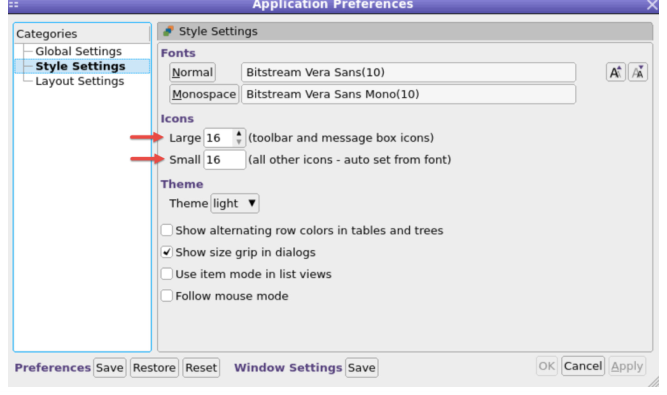
\includegraphics[width=0.92\textwidth]{gui-fig-001.png}
\caption{图标大小的应用程序首选项}
\label{fig:gui-1}
\end{figure}

\begin{figure}[htbp]
\centering
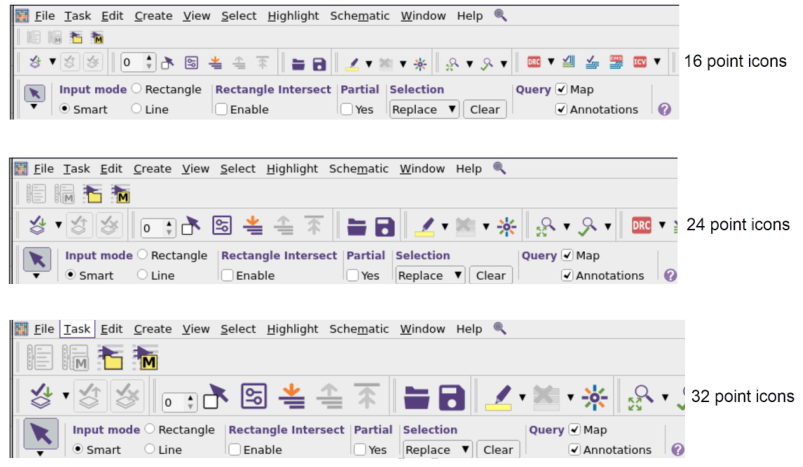
\includegraphics[width=0.92\textwidth]{gui-fig-002.png}
\caption{使用 16、24 与 32 点图标显示的工具栏}
\label{fig:gui-2}
\end{figure}

\subsection{选择浅色或深色显示主题}
\subsubsection*{Selecting a Light or Dark Display Theme}

要把背景从默认的浅灰主题改为深灰主题，选择 \textbf{View > Preferences > Style Settings}，并在 Theme 框中选择 dark。图~\ref{fig:gui-3} 同时给出浅色与深色主题。

\begin{figure}[htbp]
\centering
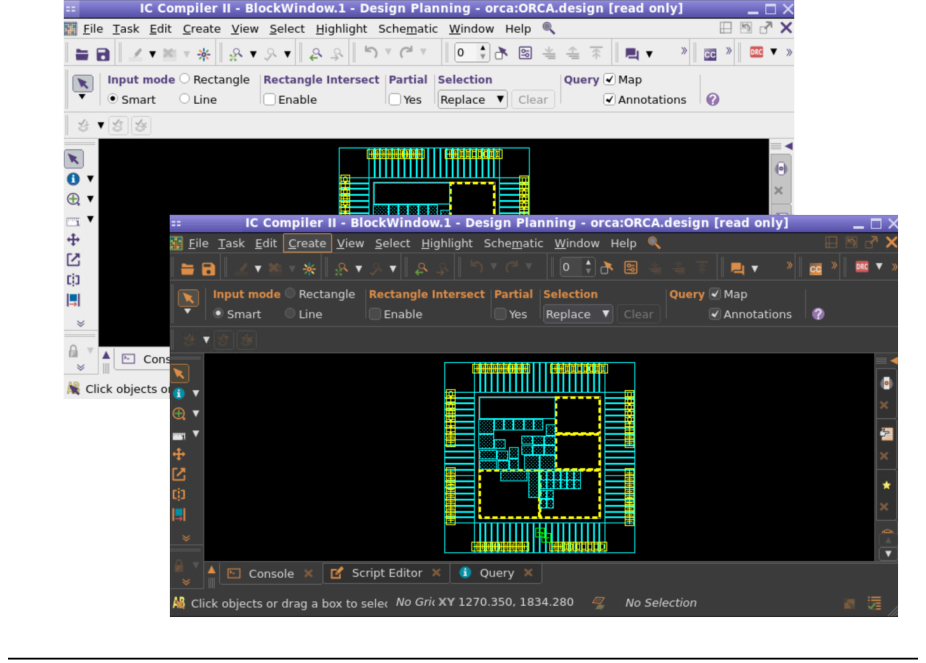
\includegraphics[width=0.92\textwidth]{gui-fig-003.png}
\caption{浅色与深色主题}
\label{fig:gui-3}
\end{figure}

% ============================================================
\section{使用命令搜索}
\subsection*{Using Command Search}

IC Compiler II GUI 提供命令搜索功能，用于快速定位菜单与任务操作、shell 命令以及应用选项。

要搜索命令：
\begin{enumerate}
  \item 单击菜单栏上的放大镜图标。
  \item 在表单顶部的 Search for: 部分单击一个或多个选项。
  \item 单击搜索框，键入命令名或主题的若干字母，或键入以空格分隔的多个词，以返回匹配结果列表。
\end{enumerate}

键入时，工具根据第 2 步所选选项，返回与搜索词相关的菜单与任务操作、shell 命令以及应用选项列表。对于 shell 命令，工具搜索命令名与命令选项列表，并按匹配质量对搜索结果排序。命令名匹配在搜索结果中的位置高于命令选项匹配。将指针移到搜索结果中的项目上，可查看包含该结果信息的信息提示（infotip），如图~\ref{fig:gui-4} 所示。

\begin{figure}[htbp]
\centering
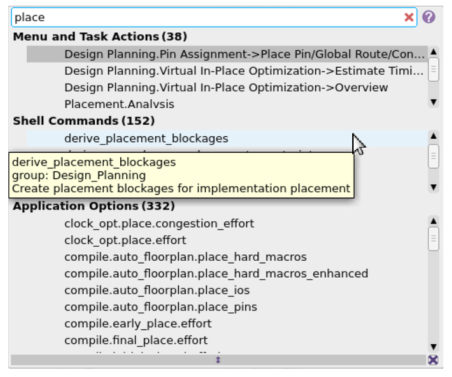
\includegraphics[width=0.92\textwidth]{gui-fig-004.png}
\caption{命令搜索结果}
\label{fig:gui-4}
\end{figure}

命令搜索支持对搜索框中一个或多个搜索词做完全匹配或部分匹配。例如，要搜索与块整形（block shaping）相关的结果，可以输入 “shape”、“block”、“sha bl”、“\cmd{shape\_blocks}” 等。若工具返回大量结果，右侧会显示滚动条以浏览列表。也可以编辑搜索词以缩小搜索结果。最后，单击列表中与搜索匹配的项目。

单击 Menu and Task Actions 列表中的项目即可运行该项。若该操作有对话框或面板，工具会打开它。若单击 Shell Commands 部分中的项目，工具会动态生成对话框。更多信息见本节「使用命令对话框（Using the Command Dialog）」。

若单击 Application Options 列表中的项目，工具打开 \textbf{Application Options} 对话框并显示所选应用选项。按需要设置该应用选项的值，单击 OK 保存更改，或单击 Cancel 保持该选项不变。也可以从菜单栏选择 \textbf{File > Application Options} 打开 \textbf{Application Options} 对话框。

使用命令搜索时，工具会记住当前工具会话中的搜索词以及你选择的操作。工具在 Recently found 部分显示以往选择的历史，在 Recently searched 部分显示本会话的搜索词。单击 Recently found 部分中的项目可再次执行该操作，或单击 Recently searched for 部分中的项目以重复该搜索。

命令搜索工具还支持下列附加功能：
\begin{itemize}
  \item 单击搜索框右侧的书本图标，用 Web 浏览器打开指向 SolvNetPlus 的链接，以搜索该搜索词。
  \item 单击搜索框右侧的 (X)，清除搜索框中的任何文本（仅当搜索框中含有文本时）。
  \item 按 Tab 键，在搜索栏与命令搜索工具的三个部分之间移动焦点。
  \item 将指针悬停在 Menu and Task Actions 部分与 Shell Commands 部分之间，或悬停在 Shell Commands 与 Application Options 部分之间，以显示分隔条；单击并拖动分隔条可调整该部分的大小。
  \item 单击并拖动命令搜索工具底部的条，以调整对话框大小。
  \item 单击命令搜索工具外部，或按 Esc 键，以关闭该工具。
\end{itemize}

\subsection{使用命令对话框}
\subsubsection*{Using the Command Dialog}

在 IC Compiler II 工具中，图形用户界面为工具中的 Tcl 命令即时生成对话框。在命令搜索的 Shell Commands 列表中单击某项时，工具为该命令生成对话框，如图~\ref{fig:gui-5} 所示。

\begin{figure}[htbp]
\centering
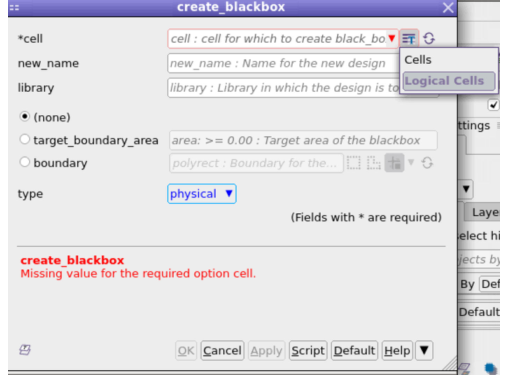
\includegraphics[width=0.92\textwidth]{gui-fig-005.png}
\caption{命令对话框}
\label{fig:gui-5}
\end{figure}

对话框在顶部列出选项与数据输入字段，在底部显示状态信息与命令预览。底行包含与此对话框相关的任务按钮。

在顶部，对话框中的必填字段以星号（*）标记。在文本框中键入时，工具校验输入。若输入中未检测到错误，工具以蓝色显示文本并更新命令预览。若输入包含错误，工具以红色显示文本，并在命令预览区域显示错误消息。单击 Default 按钮可恢复对话框中的默认值。要了解某个文本框的用途，将指针悬停在该框上以查看信息提示。

也可以在命令对话框中输入 Tcl 表达式与变量。例如，可以在图~\ref{fig:gui-5} 的 cell 文本框中输入下列内容：
\begin{itemize}
  \item 实际的单元名，例如 \cmd{u0\_0}
  \item \cmd{\$cell} 变量，用于指定你已定义的、包含单元名的变量
  \item Tcl 表达式，例如 \cmd{[get\_cells u0\_0]}
\end{itemize}

在可能的情况下，对话框提供用于选择边界框、层以及枚举值的工具，以帮助指定命令。要指定边界，执行下列操作之一：
\begin{itemize}
  \item 要定义矩形边界，选择相应按钮，然后在 Coordinates 框中输入矩形左上角与右下角的 $x$ 与 $y$ 坐标，或在版图视图中拖动指针，在所需位置形成矩形。
  \item 要定义直角多边形边界，选择相应按钮，然后在 Coordinates 框中输入每个拐角或方向变化处的 $x$ 与 $y$ 坐标，或在版图视图中拖动指针，在所需位置形成多边形各边。
  \item 要手动输入坐标，单击相应按钮，并在 Coordinates 框中输入矩形左上角与右下角的 $x$ 与 $y$ 坐标。
  \item 要启用或禁用网格吸附，选中或取消相应按钮。
  \item 要从列表中选择选项，单击相应按钮，并在出现的菜单上选择一项。
\end{itemize}

若命令选项要求指定一个或多个层，单击相应按钮并选择各层。也可以单击另一按钮并键入层名称。

若命令选项支持多个枚举值，单击相应按钮，并在出现的菜单上选择一项。对于所有其他表单输入项，在文本框中键入值。

在底部，工具提供用于执行不同操作的按钮：
\begin{itemize}
  \item 单击 OK 运行命令并关闭对话框。若对话框中存在错误，必须先纠正错误再单击 OK。
  \item 单击 Cancel 停止该命令。
  \item 单击 Apply 运行命令并保持对话框打开。
  \item 单击 Script 把命令复制到 Script Editor 窗口，而不运行该命令。
  \item 单击 Default 恢复对话框中的默认值。
  \item 单击 Help 在 Man Page Viewer 中打开该命令的 man 页。
\end{itemize}

% ============================================================
\section{使用主题搜索}
\subsection*{Using Topic Search}

工具提供界面，用于搜索安装目录中的帮助主题与其他文档。可搜索的文档包括 man 页、每日提示（tip of the day），以及通过菜单或单击按钮访问的 GUI 功能帮助主题。若搜索词包含在命令名、应用选项名、文档标题或文档关键字列表中，匹配项会出现在搜索结果中。请注意，该搜索工具不考虑通过 SolvNet 提供的在线文档。

要打开搜索工具：
\begin{enumerate}
  \item 选择 \textbf{Help > Man Pages}，打开 man 页查看器。\\
        第一次打开搜索工具时，工具显示用于查看 shell 命令、应用选项、错误消息、GUI 帮助以及每日提示主题的链接，如下图所示。
\end{enumerate}

\begin{figure}[htbp]
\centering
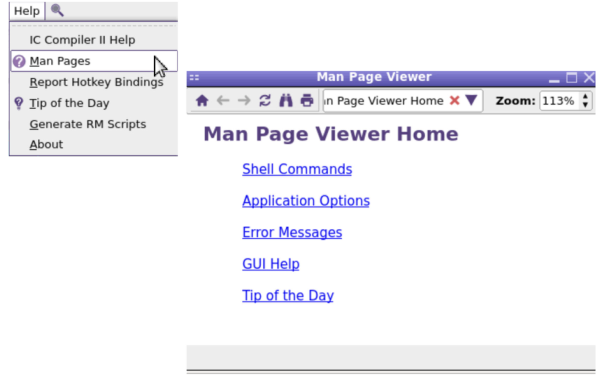
\includegraphics[width=0.92\textwidth]{gui-fig-006.png}
\caption{Man 页查看器}
\label{fig:gui-6}
\end{figure}

\begin{enumerate}
  \setcounter{enumi}{1}
  \item （可选）单击某个链接，查看该类别的目录。
  \item 在标题栏中输入搜索词，以显示与该词匹配的命令、应用选项和帮助主题。
\end{enumerate}

\begin{figure}[htbp]
\centering
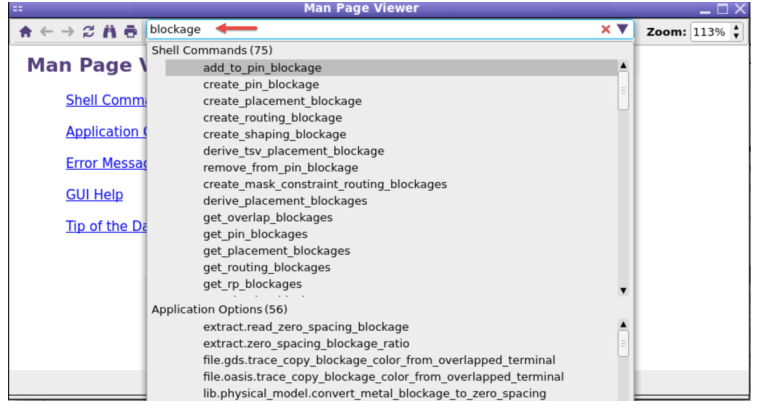
\includegraphics[width=0.92\textwidth]{gui-fig-007.png}
\caption{搜索词}
\label{fig:gui-7}
\end{figure}

\begin{enumerate}
  \setcounter{enumi}{3}
  \item 单击搜索框右侧的向下箭头，查看搜索历史。
\end{enumerate}

\begin{figure}[htbp]
\centering
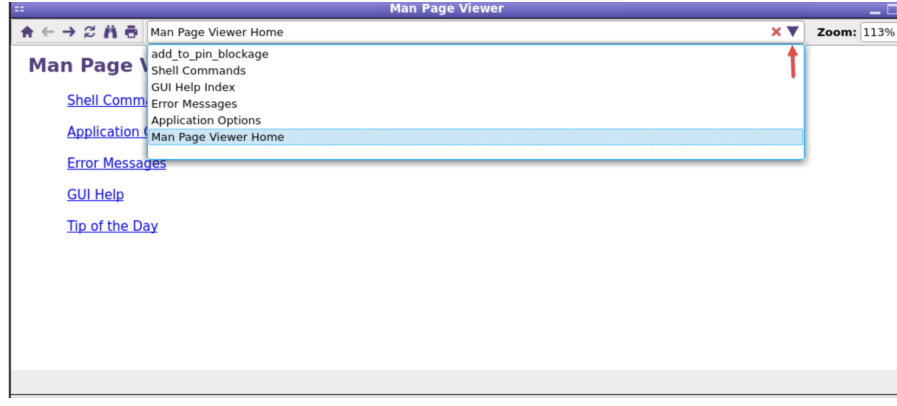
\includegraphics[width=0.92\textwidth]{gui-fig-008.png}
\caption{搜索历史}
\label{fig:gui-8}
\end{figure}

% ============================================================
\section{查看每日提示}
\subsection*{Viewing the Tip of the Day}

工具提供一组有用的提示，可用于改进工作流程。要查看每日提示，从菜单选择 \textbf{Help > Tip of the Day}。工具显示一条随机的每日提示。使用 Prev 与 Next 按钮查看更多提示。

% ============================================================
\section{创建参考方法学脚本}
\subsection*{Creating Reference Methodology Scripts}

面向 IC Compiler II 工具的 Synopsys 参考方法学（reference methodology）是一组脚本，其中收录了针对各厂商与工艺节点使用该工具的最新推荐方法。这些脚本是起点，可按你自己的设计需求加以改编和扩展。脚本中嵌有注释与备选设置，便于按需要定制流程。

要使用 GUI 为 IC Compiler II 工具生成 RM 脚本：
\begin{enumerate}
  \item 从菜单选择 \textbf{Help > Generate RM Scripts}。
  \item 为设计选择 Technology node。
  \item 为设计输入 Foundry 名称。
  \item 选择脚本的版本类型：Full RM 或 JumpStart。JumpStart 是新用户的起点，适用于已准备好执行 \cmd{place\_opt} 命令的块；这些脚本对扁平设计（flat design）运行推荐的默认布局布线（place-and-route）流程。
  \item 为脚本输入输出目录。默认情况下，压缩的 tar 文件写到当前目录。
  \item 单击 “I agree to the above Terms and Conditions.” 旁边的方框。
  \item 单击 OK。
\end{enumerate}

这些步骤把压缩的 tar 文件写到第 5 步指定的目录。写出文件后，使用 \cmd{tar xzf} \textit{filename} 命令解压文件。也可以用 \cmd{generate\_rm} 命令创建参考方法学脚本。

\begin{noteBox}
某些工艺节点需要晶圆厂提供的额外配置文件。请联系 Synopsys 代表，以获取这些文件方面的帮助。
\end{noteBox}

% ============================================================
\section{查看与编辑应用选项}
\subsection*{Viewing and Editing Application Options}

IC Compiler II 工具使用应用选项（application options）控制工具行为。为管理应用选项，IC Compiler II GUI 提供工具，用于显示当前应用选项设置、更改设置、把设置恢复为默认值，以及获取特定应用选项的帮助。

要打开应用选项工具，选择 \textbf{File > Application Options}，或在命令搜索结果中单击某个应用选项。

\begin{figure}[htbp]
\centering
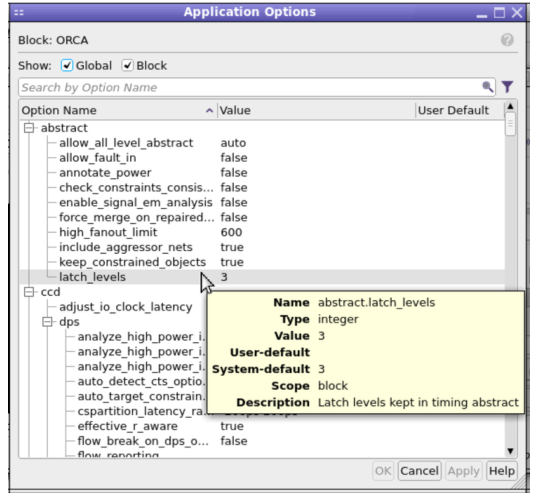
\includegraphics[width=0.92\textwidth]{gui-fig-009.png}
\caption{应用选项对话框}
\label{fig:gui-9}
\end{figure}

在 Tcl 命令中指定应用选项时，使用下列命名约定：
\begin{lstlisting}
category[.subcategory].option_name
\end{lstlisting}
其中 \cmd{category} 一般指受该应用选项影响的引擎。某些应用选项类别还有可选的子类别，用于进一步细化该应用选项所影响的范围。

应用选项具有全局作用域（global scope）或块作用域（block scope）。
\begin{itemize}
  \item 块作用域应用选项只应用于设置它们的那个块。它们保存在设计库中，并在多次工具会话之间保持。
  \item 全局作用域应用选项应用于所有块，但仅在当前会话内有效。它们不保存在设计库中；必须在每个 \cmd{icc2\_shell} 会话中指定。可以考虑把全局设置加入 \cmd{.synopsys\_icc2.setup} 文件。
\end{itemize}

\subsection{查看应用选项}
\subsubsection*{Viewing Application Options}

打开 \textbf{Application Options} 对话框后，工具显示当前的应用选项名称与设置。单击 Global 选项、Block 选项或两者，以选择要显示的应用选项作用域。要过滤应用选项列表，在搜索框中输入搜索词。键入时，工具过滤应用选项，只显示名称中包含该搜索词的选项。要按 Value 列过滤，输入 “Value:” 后接搜索词。例如，输入 “Value:true” 可只显示 Value 列中设置为 “true” 的应用选项。

要进一步限制列表中显示的应用选项，单击搜索框右侧的过滤按钮。取消 “Show if value is default”，以隐藏全部仍为默认值的应用选项设置。取消 “Show read-only”，以隐藏全部只读应用选项。

具有非默认设置的应用选项以粗体显示。将指针移到文本上可显示信息提示。信息提示给出选项名、选项类型、当前设置、用户默认设置、系统默认设置、作用域以及简短说明。

\begin{figure}[htbp]
\centering
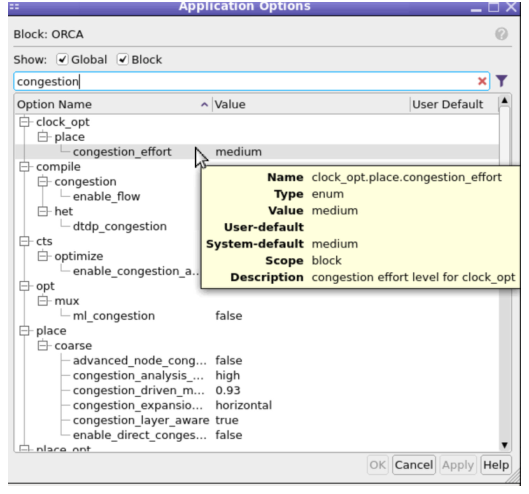
\includegraphics[width=0.92\textwidth]{gui-fig-010.png}
\caption{非默认选项}
\label{fig:gui-10}
\end{figure}

要显示某应用选项的 man 页，单击该选项以选中它，然后单击对话框右上角附近的按钮。工具打开所选应用选项的 man 页。

\subsection{编辑应用选项}
\subsubsection*{Editing Application Options}

要更改应用选项的值：
\begin{enumerate}
  \item 单击该选项值的文本。\\
        对于枚举类型与布尔类型选项，工具显示可能设置的列表。对于整数类型、浮点类型与文本选项，工具显示编辑框。
  \item 从列表中选择选项，或在文本框中输入新值。
  \item 单击 OK 保存设置并关闭对话框，或单击 Apply 保存设置。
\end{enumerate}

若应用了非默认设置，工具以粗体显示该应用选项及其设置。要把非默认设置恢复为其默认值：
\begin{enumerate}
  \item 单击选项值。
  \item 单击编辑框右侧的按钮，将该值设为其默认值。
  \item 单击 OK 或 Apply 以应用该设置。
\end{enumerate}

要把应用选项的值设为基于 Tcl 变量的值，按如下方式使用 \cmd{set\_app\_options} 与 \cmd{list} 命令：
\begin{lstlisting}
icc2_shell> set scriptdir "myscriptdir"
myscriptdir

icc2_shell> set_app_options \
   -list [list signoff.fix_drc.run_dir $scriptdir]
signoff.fix_drc.run_dir myscriptdir

icc2_shell> report_app_options signoff.fix_drc.run_dir
****************************************
Report : app_option
Design : ORCA
****************************************
Name                    Type   Value
----------------------- ------ -----------
signoff.fix_drc.run_dir string myscriptdir
----------------------- ------ -----------
1
\end{lstlisting}
